% =====================================================================
%  Bachelor's Thesis -- Innopolis University, 2026
%  "When Does Memory Help an LLM Judge? Evaluation of Memory-Augmented
%   Judging"
%
%  Structure follows the DOE recommendations and the accepted
%  Innopolis bachelor's-thesis layout:
%    Introduction, Literature Review, Methodology, Implementation,
%    Evaluation and Discussion, Conclusion, Bibliography, Appendices.
%
%  DOE formatting (re-applied on docx assembly):
%    Times New Roman 14pt, line spacing 1.5,
%    margins left 25mm / others 20mm, first-line indent 1.25cm,
%    each chapter on a new page, continuous page numbering.
% =====================================================================
\documentclass[14pt,a4paper]{extreport}

\usepackage[utf8]{inputenc}
\usepackage[T1]{fontenc}
\usepackage{times}
\usepackage[english]{babel}
\usepackage{geometry}
\geometry{a4paper, left=25mm, right=20mm, top=20mm, bottom=20mm}
\usepackage{graphicx}
\usepackage{amsmath}
\usepackage{amssymb}
\usepackage{booktabs}
\usepackage{longtable}
\usepackage{array}
\usepackage{hyperref}
\usepackage{cite}
\usepackage{setspace}
\usepackage{indentfirst}

\hypersetup{colorlinks=true, linkcolor=black, citecolor=black, urlcolor=black}

\onehalfspacing
\setlength{\parindent}{1.25cm}
\renewcommand{\ttdefault}{\rmdefault}
\renewcommand{\texttt}[1]{\textit{#1}}

\begin{document}

% =====================================================================
%  TITLE PAGE  (replaced by the official DOE template on docx assembly)
% =====================================================================
\thispagestyle{empty}
\begin{titlepage}
\begin{center}
{\bfseries Autonomous Non-Profit Organization of Higher Education\\
``Innopolis University''}
\vspace{1.0cm}

{\bfseries FINAL QUALIFICATION WORK\\(BACHELOR'S THESIS)\\
in the Academic Program 09.03.01 ``Computer Science''}
\vspace{0.5cm}

{\bfseries Field of Study: ``Data Science and Artificial Intelligence''}
\vspace{1.5cm}

{\large \textbf{Topic:}}\\[0.4cm]
{\Large \textbf{When Does Memory Help an LLM Judge?\\
Evaluation of Memory-Augmented Judging}}
\vspace{2.5cm}

\begin{flushleft}
\hspace{1cm}\begin{tabular}{@{}p{5cm}p{4cm}p{4cm}@{}}
Prepared by & \hrulefill & Khush Patel \\[1.0cm]
Supervisor & \hrulefill & Prof.\ Bader Rasheed \\
\end{tabular}
\end{flushleft}
\vfill
{\normalsize Innopolis, 2026}
\end{center}
\end{titlepage}

% =====================================================================
%  ABSTRACT
% =====================================================================
\chapter*{Abstract}
\addcontentsline{toc}{chapter}{Abstract}

Large Language Models are increasingly used as automatic judges that score the outputs of other models. This thesis investigates whether equipping an LLM judge with a persistent, structured memory of its past evaluations improves its verdicts. A memory-augmented judging system, MCTS-MAJ, was implemented, together with a leakage-free evaluation protocol and a two-layer frozen-memory audit that proves memory is not modified during evaluation. Under a conventional protocol, memory appeared to deliver large gains; under the leakage-free, audited protocol no configuration significantly outperformed a single-pass stateless judge. This null result is established for a single judge model, GPT-4o, on an eighty-sample held-out set, and is therefore stated as ``no effect was detected at this scale'' rather than as a universal claim. The audit also caught a real leakage defect, and a corrected re-run showed that a previously reported collapse under memory poisoning was a measurement artifact. The thesis explains, mechanistically, why memory neither helped nor harmed on this benchmark, and identifies the conditions under which it would be expected to help. Both the apparent benefit and the apparent fragility of memory are largely artifacts of the evaluation protocol.

\textbf{Keywords:} LLM-as-a-Judge, memory-augmented evaluation, retrieval-augmented generation, Monte Carlo Tree Search, evaluation leakage, frozen-memory audit, statistical significance, negative result.

\tableofcontents
\listoftables
\addcontentsline{toc}{chapter}{List of Tables}
\listoffigures
\addcontentsline{toc}{chapter}{List of Figures}

% =====================================================================
%  CHAPTER 1 -- INTRODUCTION
% =====================================================================
\chapter{Introduction}

\section{Relevance of the Topic}

Large Language Models (LLMs) are now used not only to generate text but also to \emph{evaluate} it. In the LLM-as-a-Judge paradigm, a language model reads a task, a candidate response, and a grading rubric, and returns a verdict \cite{mt_bench2023, geval2023, judge_survey2024}. Automatic judges rank chatbots, score the outputs of automated agents, and provide reward signals during model training. Because their verdicts increasingly drive downstream decisions, the trustworthiness of an automatic judge is a first-order research concern \cite{chateval2023, llm_judge_agreement2024}.

A standard LLM judge is \emph{stateless}: it evaluates each item in isolation and retains nothing between evaluations. It cannot recognize that it has already seen a near-identical case, cannot reuse a correct line of reasoning, and cannot learn from a past mistake. This limitation motivates \emph{memory-augmented} judging, in which the judge is connected to a persistent store of its past evaluations and retrieves relevant prior cases before producing a verdict. The idea extends retrieval-augmented generation \cite{rag_original2020} and the broader move toward language agents with long-term memory \cite{memgpt2023, generative_agents2023, reflexion2023}.

Memory, however, is double-edged. The same mechanism that supplies useful prior signal can also propagate the judge's own past errors, can be deliberately corrupted \cite{rag_poisoning2024}, and, most subtly, can leak information between related evaluation items. Benchmark contamination and evaluation leakage are recognized threats to the validity of LLM evaluation \cite{data_contamination2024, benchmark_contamination2024, eval_leakage2024}, and a memory that is updated during evaluation is a direct channel for such leakage. The topic of this thesis is therefore timely: as memory-augmented judges move toward practical use, the field needs a disciplined way to measure whether memory genuinely helps, and a way to detect when an apparent improvement is in fact an artifact of a leaky measurement.

\section{Problem Statement}

Given an LLM-as-a-Judge system, it is not currently straightforward to determine whether attaching a persistent memory improves the accuracy of its verdicts. A naive evaluation, which builds memory and tests on overlapping or paired data, or updates memory during testing, can report a large apparent gain that is caused by leakage rather than by genuine reasoning improvement. Conversely, a poorly instrumented evaluation harness can report large apparent failures that are caused by unhandled engineering faults rather than by the system under test. The problem is therefore twofold: to design an evaluation protocol that is provably free of memory leakage, and to use that protocol to obtain an honest, statistically grounded answer to the question of whether, when, and why memory helps.

\section{Purpose and Research Question}

The purpose of this work is to design, implement, and rigorously evaluate a memory-augmented LLM-as-a-Judge system, and to determine under what conditions persistent memory genuinely improves evaluation quality.

The thesis is organized around a single research question:

\begin{quote}
\textbf{When does persistent memory help an LLM-as-a-Judge, when does it fail or corrupt the evaluation, and how can a memory-augmented judge be evaluated in a provably leakage-free way?}
\end{quote}

\section{Objectives}

To answer the research question, the following objectives were set:

\begin{enumerate}
    \item Design and implement a memory-augmented judge (MAJ) that stores past evaluations in a structured, typed graph and retrieves relevant prior cases at evaluation time.
    \item Implement two exploratory extensions that apply Monte Carlo Tree Search at the reasoning layer and at the memory-retrieval layer.
    \item Design a leakage-free evaluation protocol that partitions the benchmark by question and freezes memory during testing.
    \item Implement a two-layer frozen-memory audit that proves, for every run, that memory was not modified during evaluation.
    \item Conduct controlled experiments comparing no-memory, self-written-memory, oracle-memory, and poisoned-memory conditions, with confidence intervals and paired significance tests.
    \item Determine whether the apparent effect of memory survives a leakage-free, audited protocol, and explain the result mechanistically.
\end{enumerate}

\section{Object and Subject of Research}

The \textbf{object} of research is the LLM-as-a-Judge evaluation process: the procedure by which a language model assigns a pass/fail verdict to a candidate response under a grading rubric. The \textbf{subject} of research is the effect of a persistent, retrieval-conditioned memory on the accuracy and the measurement validity of that process, together with the protocol required to measure that effect without leakage.

\section{Scientific Novelty}

The scientific novelty of this thesis consists of the following.

\begin{enumerate}
    \item \textbf{MCTS-MAJ as a research platform.} The thesis designs and implements MCTS-MAJ, a memory-augmented LLM-as-a-Judge built on a typed graph of past evaluations with a three-stage retrieval pipeline and two Monte Carlo Tree Search components. While memory-augmented and tree-search judging build on existing directions, the integrated system serves as the controlled platform on which the leakage question below is studied; it is, to date, the first memory-augmented judge whose evaluation is explicitly designed to be audited for leakage.
    \item \textbf{The first provably leakage-free, audited evaluation of a memory-augmented LLM judge.} Question-level data splitting and state hashing are individually established techniques; the novelty here is their combination into a protocol applied, for the first time, to memory-augmented LLM-as-a-Judge systems, and made \emph{provable} rather than assumed. The two-layer frozen-memory audit (a deterministic before-and-after snapshot with a SHA-256 fingerprint over the graph contents, together with runtime interception of every memory-write operation) is the first known evaluation harness for memory-augmented judging that proves, rather than assumes, the absence of memory leakage.
    \item \textbf{A corrective empirical finding.} Applying the audited protocol overturns a previously plausible result: the large apparent benefit of memory observed under a conventional protocol does not survive, and on the studied benchmark no memory-augmented or tree-search configuration significantly outperforms a single-pass stateless judge. The thesis further explains this finding mechanistically.
    \item \textbf{A methodological demonstration.} An un-audited harness can report effects that do not exist, both an apparent accuracy gain and an apparent catastrophic poisoning collapse, and an audited, error-handling-correct harness removes both artifacts. This establishes the audited protocol as a necessary precondition for trustworthy claims about memory-augmented judging.
\end{enumerate}

\section{Practical Significance}

The leakage-free protocol and the frozen-memory audit form a small, self-contained instrument that any practitioner building a memory-augmented LLM judge can apply to obtain trustworthy measurements. The empirical finding is a cautionary result for practitioners: an apparent improvement from memory should not be believed until the evaluation has been audited for leakage and instrumented for transient failures. The complete implementation, including the audit, the statistical pipeline, and a one-command reproduction script, is released so that the protocol can be adopted directly.

\section{Structure of the Thesis}

Chapter~2 reviews the literature on LLM-as-a-Judge, retrieval- and memory-augmented systems, Monte Carlo Tree Search, evaluation validity, and statistical methods. Chapter~3 presents the methodology: the MCTS-MAJ architecture, the leakage-free protocol, and the frozen-memory audit. Chapter~4 describes the implementation. Chapter~5 reports and discusses the experimental results, organized around when memory appears to help, when it fails or misleads, and how it is audited. Chapter~6 concludes the thesis and outlines future work.

% =====================================================================
%  CHAPTER 2 -- LITERATURE REVIEW
% =====================================================================
\chapter{Literature Review}

\section{LLM-as-a-Judge Evaluation}

LLM-as-a-Judge refers to the use of a large language model to assess the quality of a response produced by another model or by a human \cite{mt_bench2023, geval2023}. The judge is given a task description, a candidate response, and a grading rubric, and it returns a verdict, usually with a short justification. The appeal of the paradigm is scale: an LLM judge can score thousands of items at a fraction of the cost and latency of human annotation, and systems such as G-Eval \cite{geval2023} and Prometheus \cite{prometheus2023} report high agreement with human raters on several tasks.

The paradigm also has well-documented weaknesses. LLM judges exhibit systematic biases: they can be sensitive to the position of a response in a pairwise comparison, to response length, to self-preference, and to superficial stylistic features \cite{llm_judge_bias2024, position_bias2024}. Recent work on the reliability of LLM-based evaluators \cite{chateval2023, llm_judge_agreement2024} emphasize that automatic judges must themselves be evaluated carefully, that headline agreement numbers are often fragile, and that judge verdicts can be poorly calibrated \cite{judge_calibration2024}. A stateless judge, in particular, has no mechanism to be consistent across related items, because it does not remember how it judged a similar case a moment earlier. This limitation is the entry point for memory augmentation.

\section{Retrieval-Augmented and Memory-Augmented Systems}

Retrieval-Augmented Generation (RAG) \cite{rag_original2020} extends a language model with an external store of documents that can be queried at inference time, so that the model's output is conditioned on retrieved evidence rather than on parametric knowledge alone. Subsequent work made retrieval adaptive: Active RAG \cite{active_rag2023} reformulates the retrieval query as reasoning proceeds, and Self-RAG \cite{self_rag2023} lets the model critique and selectively use its retrieved context.

A related line of work gives language agents an explicit long-term memory. MemGPT \cite{memgpt2023} treats memory management as an operating-system-like problem. Generative Agents \cite{generative_agents2023} maintain a memory stream of past observations and retrieve from it by recency, importance, and relevance. Reflexion \cite{reflexion2023} stores verbal self-feedback from past attempts so that an agent can improve on later ones. A recurring concern in this line of work is that stored content can become stale, wrong, or adversarially corrupted, a risk made concrete by knowledge-corruption attacks on retrieval stores \cite{rag_poisoning2024}.

Applying this idea to judging, a memory-augmented judge retrieves \emph{past evaluations} rather than documents or episodes, and uses them as contrastive or confirmatory references. The present work differs from prior memory systems in two respects: the memory is organized as a \emph{typed graph} rather than a flat store, enabling structured multi-hop retrieval; and the memory is studied specifically as a potential source of \emph{evaluation leakage}, which prior memory-augmented work does not address.

\section{Monte Carlo Tree Search and Test-Time Reasoning}

Monte Carlo Tree Search (MCTS) is a heuristic search algorithm that incrementally builds a decision tree through repeated simulation \cite{uct2006, mcts_survey2012}. Each iteration performs four steps (selection, expansion, simulation, and backpropagation), and the Upper Confidence Bound for Trees (UCT) rule balances exploitation of high-reward branches against exploration of less-visited ones. MCTS is best known for game playing, most famously as a component of AlphaGo \cite{alpha_go2016}.

Recent work adapts test-time search to LLM reasoning, a direction surveyed under the heading of test-time compute scaling \cite{test_time_scaling2024}. Chain-of-Thought prompting \cite{chain_of_thought2022} showed that decomposing a problem into intermediate steps improves accuracy; Self-Consistency \cite{self_consistency2023} samples multiple reasoning paths and takes a majority vote; Tree of Thoughts \cite{tree_of_thoughts2023} explores a tree of partial solutions; and ReAct \cite{react2023} interleaves reasoning with actions. MCTS-Judge \cite{mcts_judge2025} applies MCTS directly to judging for code-correctness evaluation, treating each tree node as an evaluation subtask. The MCTS components in this thesis follow this line, but are reported as exploratory: as Chapter~5 shows, they do not yield a statistically significant accuracy gain on the studied benchmark.

\section{Evaluation Validity, Contamination, and Leakage}

A recurring theme in recent evaluation research is that measured performance can be inflated by contamination, that is, overlap between the data used to build a system and the data used to test it. Surveys of data contamination \cite{data_contamination2024} and studies of benchmark contamination \cite{benchmark_contamination2024, eval_leakage2024} show that test items appearing, directly or indirectly, in training or memory can substantially inflate reported scores. For retrieval systems specifically, knowledge-corruption attacks such as PoisonedRAG \cite{rag_poisoning2024} demonstrate that injecting a small amount of false content into a retrieval store can change a system's outputs.

For a memory-augmented judge, two leakage channels are particularly relevant. The first is \emph{paired-item leakage}: many benchmarks contain closely related items, for example a passing and a failing answer to the same question, and if one item is in memory while its partner is in the test set, the judge can effectively see the answer. The second is \emph{write-back leakage}: if the memory is updated during evaluation, the verdict on an early test item becomes available when scoring a later, related one. The methodology of this thesis is designed to close both channels and, crucially, to \emph{prove} that they are closed rather than merely assert it. This proof-oriented stance distinguishes the present work from prior memory-augmented evaluation, which typically assumes the absence of leakage.

\section{Statistical Methods for Evaluation}

Because LLM judges are stochastic and benchmarks are finite, point estimates of accuracy can be misleading. This thesis reports every accuracy with a two-sided Wilson confidence interval \cite{wilson1927}, which is well behaved for proportions at moderate sample sizes. Mode-versus-mode comparisons are made on paired data, the same test items judged by both modes, and assessed with the exact McNemar test \cite{mcnemar1947}, which conditions on the discordant pairs, together with a paired bootstrap confidence interval on the accuracy difference \cite{bootstrap1993}. A difference is called statistically significant only when the McNemar p-value is below 0.05 and the bootstrap interval excludes zero. This conservative, paired methodology makes it possible to distinguish a genuine effect from sampling noise at the sample sizes used here. Negative and null results, reported with this level of rigour, are treated in this thesis as legitimate and valuable scientific outcomes.

\section{Summary}

The literature establishes three points that frame this thesis. First, LLM-as-a-Judge is useful but fragile, and automatic judges must themselves be evaluated with care. Second, memory augmentation is a natural and active idea, but existing memory-augmented systems do not treat memory as a leakage risk. Third, contamination and leakage are known to inflate evaluation results, yet there is no standard, proof-oriented protocol for evaluating a memory-augmented judge without leakage. The remainder of the thesis fills that gap.

% =====================================================================
%  CHAPTER 3 -- METHODOLOGY
% =====================================================================
\chapter{Methodology}

\section{Overview}

This chapter presents the methodology used to design and evaluate the MCTS-MAJ system. It describes the typed memory graph and the memory-assisted judge, the two exploratory Monte Carlo Tree Search components, the leakage-free evaluation protocol, the frozen-memory audit, the memory conditions, and the statistical methods. It closes with the limitations and ethical considerations of the approach.

\section{System Architecture}

The MCTS-MAJ system has three components that operate on a shared memory graph: the Memory-Assisted Judge (MAJ), the MCTS-Judge, and the MCTS-Retrieval module. They combine into a small number of evaluation modes that serve as ablations.

\subsection{The Typed Memory Graph}

Memory is stored in a Neo4j graph database \cite{neo4j2023}. Unlike a flat document store, the graph uses five typed node kinds: \textbf{Policy} (a task or grading criterion), \textbf{Attempt} (a candidate response with its verdict and reasoning), \textbf{Issue} (a specific problem identified in an attempt), \textbf{Fix} (a corrective action that resolves an issue), and \textbf{Semantic} (an abstract category that groups similar issues). Typed relationships connect them: \emph{SATISFIES} (Attempt to Policy), \emph{CAUSES} (Attempt to Issue), \emph{RESOLVES} (Fix to Issue), and \emph{ABSTRACTS\_TO} (Issue to Semantic). Every node carries a 1536-dimensional embedding of its text content, produced by the text-embedding-ada-002 model \cite{openai_embeddings2024}, and the graph maintains Hierarchical Navigable Small World vector indexes \cite{hnsw2018} for efficient similarity search.

\subsection{The Memory-Assisted Judge}

The Memory-Assisted Judge is a single-pass judge whose prompt is conditioned on retrieved memory. Retrieval proceeds in three stages: it finds the most similar past attempts, split into a positive and a negative set so that the judge sees a balanced contrastive signal; it retrieves issues semantically similar to the response under evaluation; and it aggregates recurring issue categories. Similarity thresholds are set asymmetrically (positive at least 0.85, negative at least 0.92) so that low-relevance items are dropped before they reach the judge. The retrieved material is formatted into a context block and supplied to the judge alongside the task and the response.

\subsection{Exploratory MCTS Components}

Two extensions apply Monte Carlo Tree Search and are reported as exploratory. \textbf{MCTS-Judge} decomposes an evaluation into five to seven task-specific subtasks generated by a planning step, and searches over reasoning trajectories using a UCT rule combined with an LLM self-assessment; the final verdict aggregates the best trajectory. \textbf{MCTS-Retrieval} replaces the fixed three-stage retrieval with a tree search over seven retrieval actions, including four multi-hop graph traversals, scored by the relevance, diversity, and volume of the material retrieved. These components are described for completeness; Chapter~5 shows they do not produce a statistically significant accuracy gain, and the thesis does not claim a benefit for them.

\subsection{Evaluation Modes}

The components combine into the evaluation modes used as ablations: \emph{Stateless} (single-pass judge, no memory); \emph{MAJ} (single-pass judge with memory retrieval); \emph{MCTS-Judge} (tree-search reasoning, no memory); and \emph{MCTS-Judge~+~Memory} (tree-search reasoning with memory retrieval). Comparing these isolates the contribution of memory and of tree search.

\section{The Leakage-Free Evaluation Protocol}

\subsection{The Leakage Problem}

The benchmark used in this work, EvalsBench \cite{evalsbench2024}, contains paired items: for each question there is a passing and a failing response. This pairing creates two leakage channels. If the split is made at the level of individual rows, one version of a question may land in the memory-building set and the other in the test set, so the judge effectively sees the answer. If memory is updated during testing, the verdict on an early item becomes visible when a later, related item is scored. Either channel can inflate measured accuracy without any genuine improvement in judging.

\subsection{Question-Level Partition}

To close the first channel, the benchmark is split \emph{by question}, not by row. The unique questions are shuffled with a fixed random seed and divided into a memory-building half and a test half; both the passing and the failing version of any given question always remain in the same half. No question, in any form, appears in both the memory and the test sets.

\subsection{Frozen Memory During Evaluation}

To close the second channel, the memory graph is \emph{frozen} for the duration of test evaluation. The judge may read from memory, but no node or relationship is created, modified, or deleted while the test set is being scored. Memory is built once, before evaluation, and is read-only thereafter.

\section{The Frozen-Memory Audit}

A protocol that states memory is frozen is not enough; the absence of writes must be proven for every run. The frozen-memory audit provides this proof in two independent layers.

\subsection{Layer One: Snapshot and Fingerprint}

Immediately before and immediately after evaluation, a deterministic snapshot of the graph is taken. Each snapshot records the number of nodes of each type, the number of relationships of each type, and a SHA-256 fingerprint computed over the sorted list of node identifiers and edge triples. The two snapshots are compared: the run is reported as leakage-free only if the node and relationship counts are identical and the two fingerprints match exactly. The full before-and-after record is written to a per-run audit file, so the proof is preserved and independently checkable.

\subsection{Layer Two: Runtime Write-Blocking}

The snapshot check detects leakage after the fact. The second layer prevents it. For the duration of evaluation, every write method of the graph interface (node creation, relationship creation, get-or-create, and clear) is intercepted and replaced with a guard that raises a FrozenMemoryViolation exception if called. Any code path that attempts to write to memory during evaluation therefore fails immediately and loudly, rather than corrupting the run silently.

\subsection{Value of the Audit}

The audit was not a formality. When it was first applied to the MCTS-Judge~+~Memory mode, it failed: the evaluation path was writing the just-judged test item back into memory. This is exactly the write-back leakage the protocol is designed to exclude. The defect was found because the audit raised a violation, and it was fixed by adding a read-only evaluation mode. Every result reported in Chapter~5 has a passing audit record.

\section{Memory Conditions}

To study how the source and quality of memory affect the judge, four memory-building conditions are defined. In the \textbf{no-memory} condition the graph is empty and the judge is stateless. In the \textbf{self-written} condition the judge is run on the memory-building set and its own verdicts, reasoning, issues, and fixes are stored; this is how memory would grow in real deployment, and it includes the judge's own errors. In the \textbf{oracle} condition the ground-truth labels are stored directly without running the judge, giving a memory that is guaranteed correct. In the \textbf{poisoned} condition oracle memory is used but a fixed fraction of labels (10\%, 20\%, or 50\%) is deterministically flipped, so the effect of corrupted memory can be measured.

\section{Statistical Methodology}

Every accuracy is reported with a two-sided Wilson 95\% confidence interval \cite{wilson1927}. Mode-versus-mode comparisons are computed on paired data, the identical test items judged by both modes, and assessed with the exact McNemar test \cite{mcnemar1947} and a paired bootstrap 95\% confidence interval with 10{,}000 resamples \cite{bootstrap1993}. A difference is declared statistically significant only when the McNemar p-value is below 0.05 and the bootstrap interval excludes zero. This conservative rule guards against over-claiming at the sample sizes used. Where transient errors caused a sample to fail after retries, that sample is excluded and the number of completed samples is reported alongside the accuracy.

\section{Limitations of the Methodology}

Three limitations are stated in advance. First, the held-out test set contains eighty samples; a single misclassification shifts accuracy by 1.25 percentage points, so the study can detect only moderate-to-large effects, and a null result means ``no effect was detected,'' not ``no effect exists.'' Second, the audited experiments use a single judge model, GPT-4o; a weaker or a stronger model may behave differently. Third, the benchmark is a single domain, graded question answering, so the conclusions are stated for that setting.

\section{Ethical Considerations}

EvalsBench is a public-style benchmark with no personally identifying information, so no privacy concern arises from the data. The principal ethical commitment of the work is to measurement honesty: results are reported as they are, including the finding that the system does not produce a significant gain, and including the discovery that an earlier reported effect was an artifact. All code, prompts, configurations, per-sample results, audit records, and a one-command reproduction script are released so that every number in the thesis can be independently checked.

% =====================================================================
%  CHAPTER 4 -- IMPLEMENTATION
% =====================================================================
\chapter{Implementation}

\section{Codebase}

The system is implemented in Python. The module \emph{models.py} defines the typed node data classes and an embedding helper; \emph{graph\_manager.py} manages the Neo4j connection, the vector indexes, the typed create and link operations, and the audit primitives (snapshot, diff, and the write-blocking context manager); \emph{judge.py} implements the single-pass judge used both statelessly and with memory; \emph{mcts\_judge.py} and \emph{mcts\_retrieval.py} implement the two exploratory search components; and \emph{mcts\_pipeline.py} composes the evaluation modes. The driver \emph{benchmark\_leakage\_free.py} runs the leakage-free benchmark, including the audit wrapper and the transient-error handling. The analysis scripts \emph{analyze\_stats.py}, \emph{make\_figures.py}, and \emph{reproduce\_all.py} regenerate every statistic and figure and verify every artifact.

\section{Building the Memory Graph}

For self-written memory, the judge is run on each memory-building sample and its verdict, reasoning, issues, and fixes are committed to the graph, with each issue classified into a Semantic category by a separate model call. For oracle memory, each sample yields a Policy and an Attempt whose success flag is set to the dataset ground-truth label, with no judge call, so the graph is guaranteed label-correct. For poisoned memory, oracle memory is built and then a deterministic fraction of the stored labels is flipped using a fixed seed, so the same subset is corrupted across runs.

\section{Structured Outputs}

An early version of the MCTS-Judge extracted decisions with regular expressions over free-text model output. This failed silently on roughly 15--20\% of responses that did not follow the expected template. All decision-extracting calls were migrated to a schema-validated structured-output interface \cite{pydantic2024}, which eliminated parse failures without changing the semantics of any step.

\section{Handling Transient Failures}

LLM evaluation is network-bound. In an early run, a mid-evaluation network outage caused a block of samples to error, and the original code recorded each errored sample as an incorrect answer, silently depressing accuracy. Two corrections were made. An exponential-backoff retry wrapper was added around every model call. And the error handling was changed so that a sample that still fails after retries is recorded with a null verdict and excluded from the accuracy computation, rather than counted as wrong. As Chapter~5 shows, this correction is material: it is the difference between an apparent catastrophic collapse and the true, flat result.

\section{Reproduction Pipeline}

The benchmark driver builds memory for a chosen condition, runs the leakage-free evaluation with the frozen-memory audit enabled, and writes per-sample result files together with the audit records. The analysis script recomputes the Wilson intervals, the paired bootstrap intervals, and the exact McNemar tests from those per-sample files. The figure script regenerates every figure. A single reproduction script chains these steps, verifies that every expected result file and audit record is present, confirms that every audit passed, and exits with an error if any artifact is missing or any audit failed. Running that one script regenerates the entire empirical content of Chapter~5 from the raw per-sample data.

% =====================================================================
%  CHAPTER 5 -- EVALUATION AND DISCUSSION
% =====================================================================
\chapter{Evaluation and Discussion}

\section{Dataset}

All experiments use EvalsBench \cite{evalsbench2024}, an open benchmark released by Vibrant Labs AI under the Apache-2.0 licence, designed specifically to evaluate how well a Large Language Model performs as a judge of question-answer pairs. The benchmark is distributed as a single comma-separated file, \emph{benchmark\_df.csv}, and contains no personally identifying information.

The dataset comprises 160 samples covering 80 distinct topics in the startup and financial-analysis domain, for example pre-money valuation techniques, discounted-cash-flow analysis, and comparable-company analysis. Each row has six fields: the \emph{topic}, the \emph{question}, a set of \emph{grading notes} that act as the rubric, the ground-truth \emph{target} label (pass or fail), the candidate \emph{response} under evaluation, and an optional \emph{notes} field. The grading notes mark which points are critical and which are merely important, giving the judge a structured rubric to reason against.

Two properties of EvalsBench are central to this thesis. First, the target distribution is exactly balanced: 80 passing and 80 failing responses, so accuracy is not inflated by a skewed prior. Second, and more importantly for the methodology, the benchmark is built around \emph{paired} items. The 160 samples correspond to 80 unique questions, and each question appears twice, once with a passing response and once with a failing one. This pairing is what makes EvalsBench a natural stress test for evaluation leakage: if a passing and a failing version of the same question are split across the memory and the test sets, a memory-augmented judge can effectively retrieve the answer to the item it is scoring. The leakage-free protocol of Chapter~3 is designed precisely to neutralise this risk.

\section{Experimental Setup}

Under the leakage-free protocol the benchmark is split by question into 40 memory-building questions (80 samples) and 40 test questions (80 samples), with the random seed fixed at 42 unless stated otherwise. The judge model is GPT-4o. The MCTS modes use two rollouts and a maximum depth of three; an earlier sweep to four rollouts and depth five gave no accuracy benefit at roughly four times the cost.

\section{When Memory Appears to Help: The Conventional Protocol}

Before the leakage-free protocol was designed, the MAJ core was characterized under a conventional protocol in which memory could be updated during evaluation and the paired questions were not separated. Under that protocol memory appeared to help substantially: on a curated set of structured tasks the memory-assisted judge appeared to lift accuracy from 90\% to 100\%; across judge models, memory appeared to add six to ten percentage points for capable models while adding nothing for a weak one; and seeding the memory with 100 ground-truth examples appeared to raise cold-start accuracy from 78\% to 91\%.

These observations were obtained before the leakage-free protocol existed, and the per-sample logs for them were not retained; they are reported here as the \emph{motivating observation} of the thesis rather than as verified claims. Several of the conventional-protocol configurations either update memory during evaluation or do not separate paired questions, and each of those is a leakage channel. The conventional protocol therefore establishes only that, under a naive evaluation, memory \emph{appears} to help. The decisive question, whether the gain survives a leakage-free, audited protocol, is answered in the remainder of this chapter.

\section{When Memory Fails to Help: The Leakage-Free Results}

All results in this section use GPT-4o on 80 held-out samples with the memory graph frozen and the audit passing. Accuracies are reported with Wilson 95\% confidence intervals; comparisons are paired, with McNemar tests and bootstrap intervals.

\subsection{Clean-Memory Comparison}

\begin{table}[h]
\centering
\caption{Clean-memory results: leakage-free, audited, GPT-4o.}
\label{tab:clean}
\begin{tabular}{lccc}
\toprule
Mode & Accuracy [95\% CI] & $n$ & Mean latency \\
\midrule
Stateless & 70.0\% [59.2, 78.9] & 80 & 3.6 s \\
MAJ (self-written memory) & 65.0\% [54.1, 74.5] & 80 & 4.5 s \\
MCTS-Judge (no memory) & 70.0\% [59.2, 78.9] & 80 & 31.8 s \\
MCTS-Judge + Memory & 71.8\% [61.0, 80.6] & 78 & 33.3 s \\
\bottomrule
\end{tabular}
\end{table}

Table~\ref{tab:clean} shows the four modes under clean, self-written memory. The four confidence intervals overlap substantially. The paired comparisons confirm that no difference is significant: MAJ versus stateless is $-5.0$ points (bootstrap CI $[-12.5, +1.3]$, McNemar $p=0.29$); MCTS-Judge versus stateless is exactly $0.0$ points; MCTS-Judge~+~Memory versus stateless is $+1.8$ points (McNemar $p=0.80$). The single-pass stateless judge matches or exceeds every memory-augmented and tree-search configuration within statistical confidence.

\begin{figure}[h]
\centering
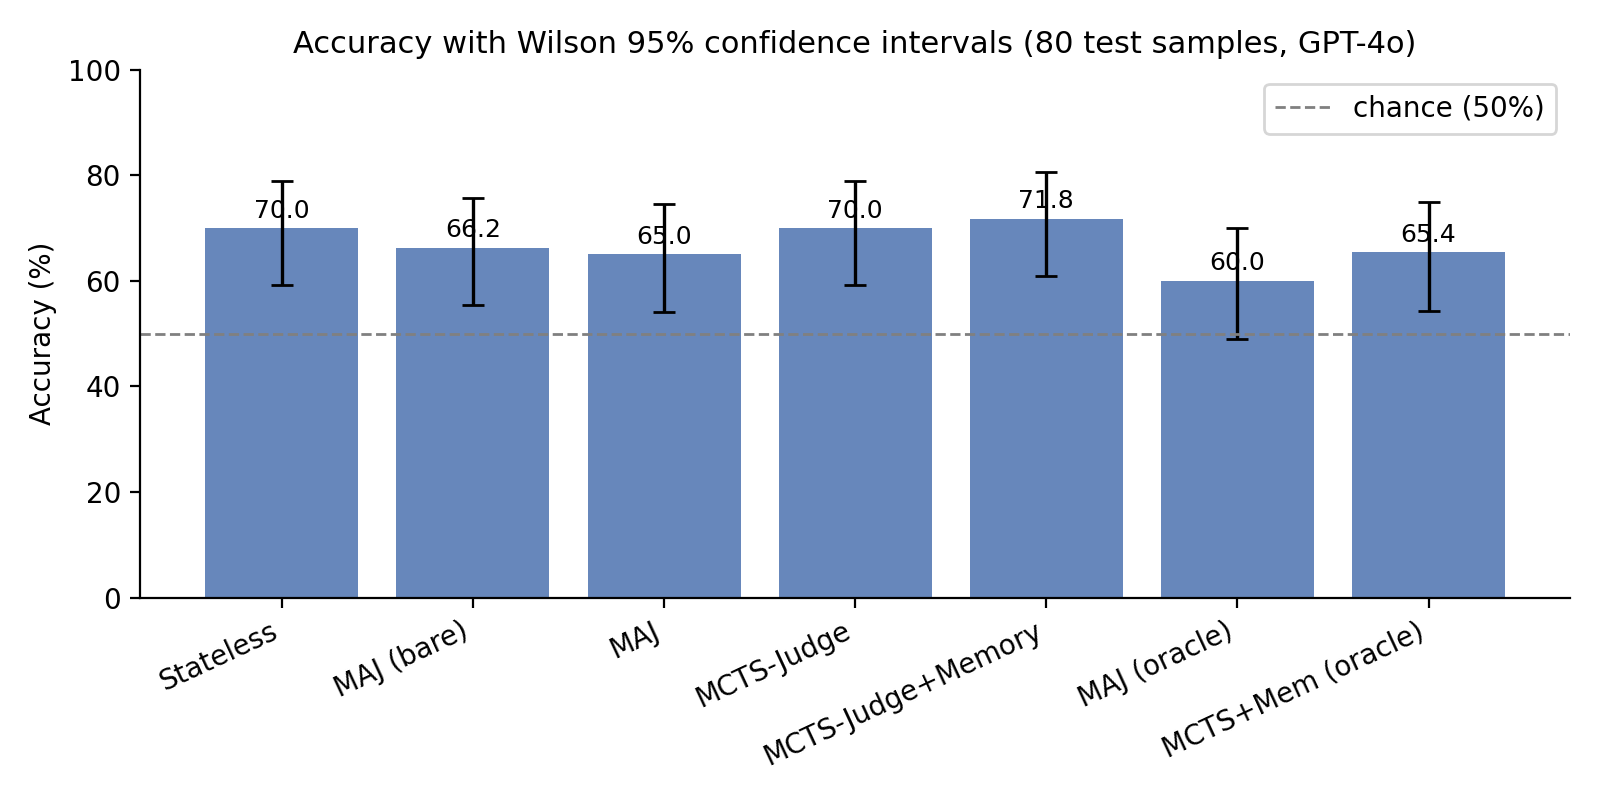
\includegraphics[width=0.95\textwidth]{figures/accuracy_ci.png}
\caption{Per-mode accuracy with Wilson 95\% confidence intervals on the leakage-free, audited test set. The error bars of every mode overlap with those of the stateless baseline.}
\label{fig:accuracy}
\end{figure}

Figure~\ref{fig:accuracy} presents the same data with confidence intervals drawn explicitly; the overlap of every interval with the stateless interval is the visual form of the central finding. Figure~\ref{fig:deltas} shows the paired mode-versus-mode differences as a forest plot; every interval that involves a clean-memory comparison crosses zero.

\begin{figure}[h]
\centering
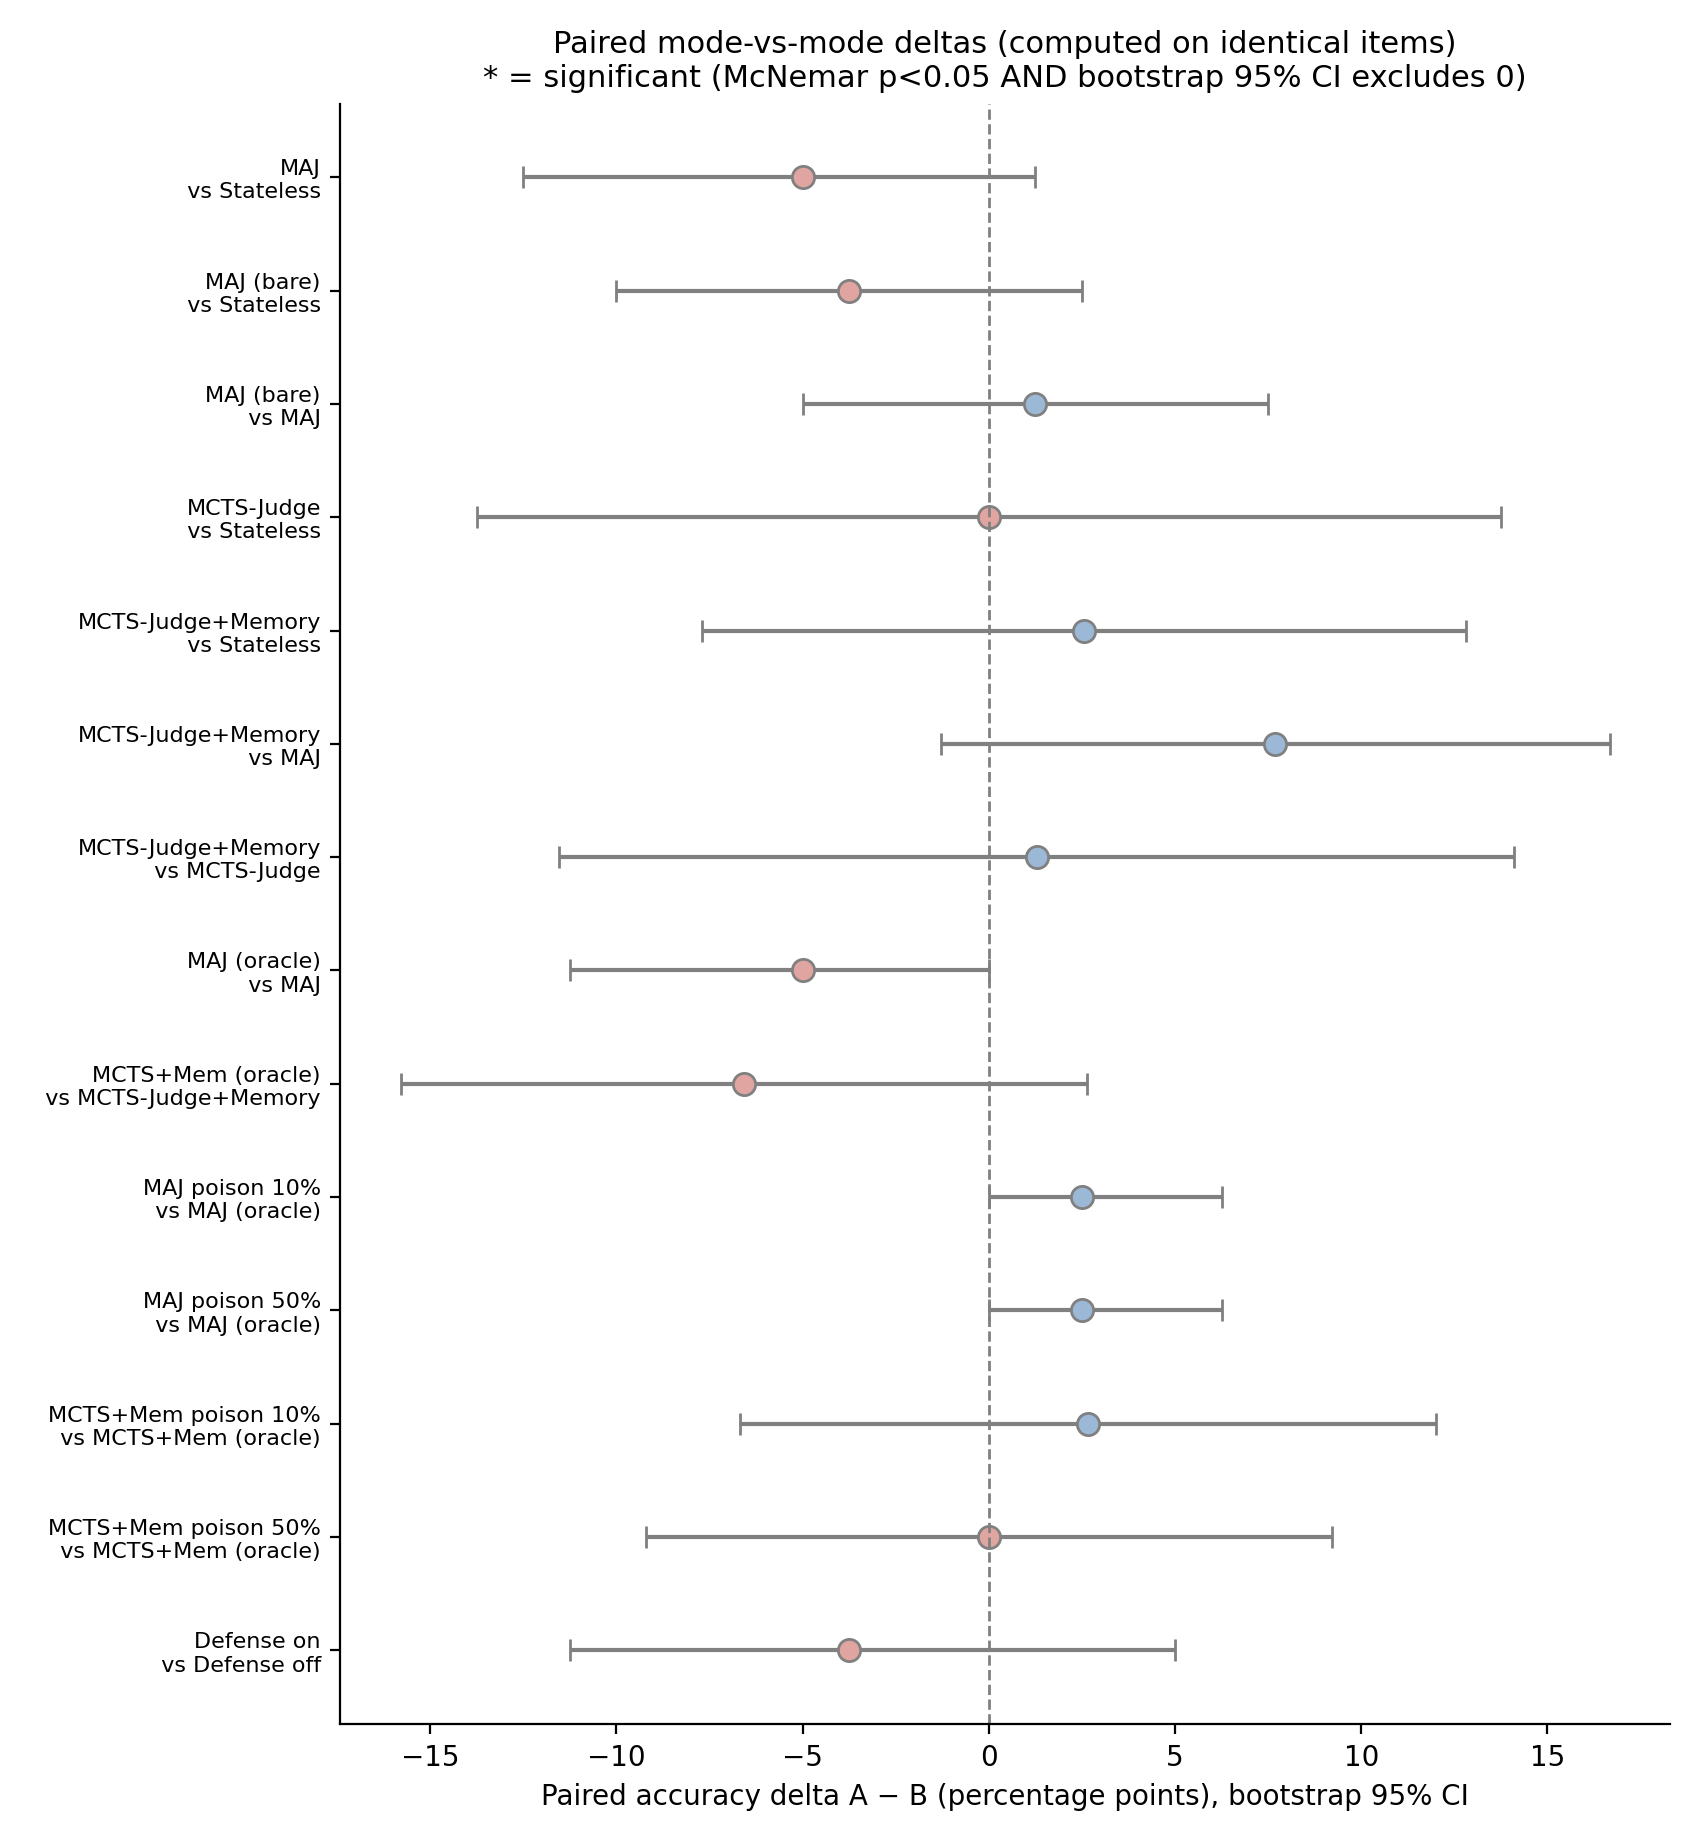
\includegraphics[width=0.95\textwidth]{figures/paired_deltas.png}
\caption{Paired accuracy differences between modes, computed on identical items, with bootstrap 95\% confidence intervals. An interval crossing the dashed zero line indicates a non-significant difference; all clean-memory comparisons do so.}
\label{fig:deltas}
\end{figure}

This is the central result: under a leakage-free, audited protocol, the apparent benefit of memory observed under the conventional protocol does not appear.

A closer look at the per-mode error structure reinforces the point. Figure~\ref{fig:confusion} shows the 2x2 confusion matrices for the four modes, and Figure~\ref{fig:passfail} splits accuracy by ground-truth class. All four modes share the same characteristic error profile: they are markedly more accurate on passing responses than on failing ones, a pass-oriented bias that memory and tree search do not correct. If memory were contributing genuine evaluative signal, it would be expected to shift this class-conditional error structure; it does not. The error profile is a property of the underlying judge model, not of whether memory is attached.

\begin{figure}[h]
\centering
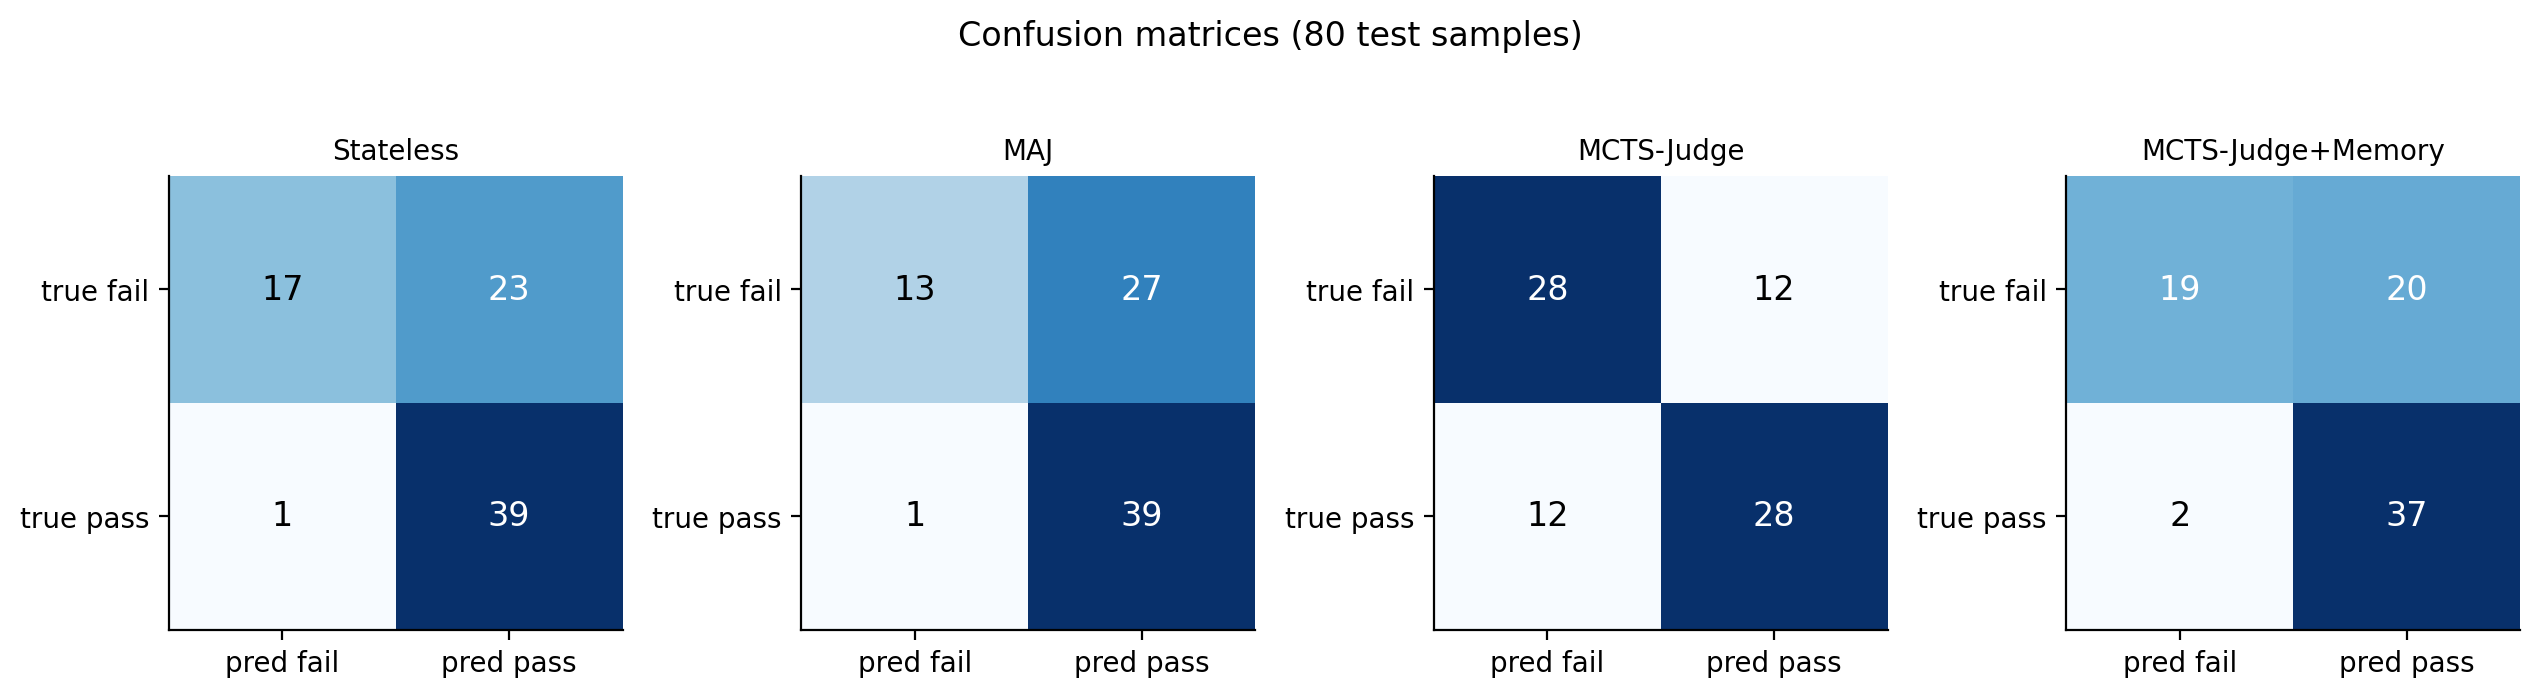
\includegraphics[width=0.95\textwidth]{figures/confusion_matrices.png}
\caption{Per-mode confusion matrices on the leakage-free test set. The four modes share the same error structure, with more errors on failing responses than on passing ones.}
\label{fig:confusion}
\end{figure}

\begin{figure}[h]
\centering
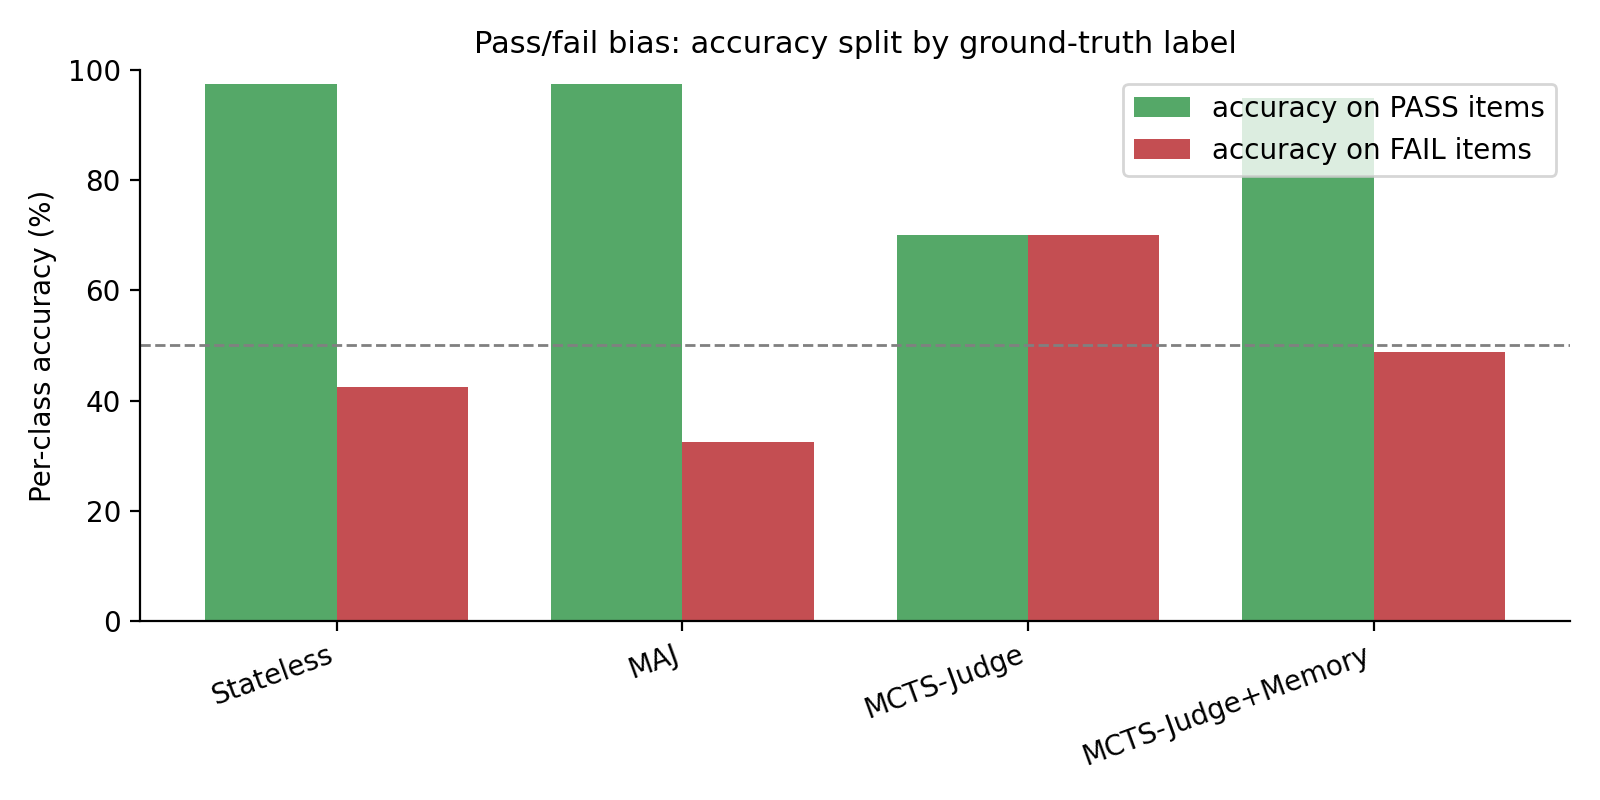
\includegraphics[width=0.95\textwidth]{figures/passfail_bias.png}
\caption{Per-class accuracy split by ground-truth label. Every mode is more accurate on passing responses than on failing ones; attaching memory does not correct this pass-oriented bias.}
\label{fig:passfail}
\end{figure}

\subsection{Self-Written versus Oracle Memory}

\begin{table}[h]
\centering
\caption{Effect of memory provenance (leakage-free, audited).}
\label{tab:oracle}
\begin{tabular}{lcc}
\toprule
Memory provenance & MAJ & MCTS-Judge + Memory \\
\midrule
Self-written & 65.0\% & 71.8\% \\
Oracle (ground-truth) & 60.0\% & 65.4\% \\
\bottomrule
\end{tabular}
\end{table}

Replacing self-written labels with perfectly correct oracle labels does not improve either mode (Table~\ref{tab:oracle}); both are slightly lower with oracle memory, and neither difference is significant (MAJ $-5.0$ points, $p=0.22$; MCTS-Judge~+~Memory $-6.6$ points, $p=0.27$). This is itself informative. If the judge were genuinely exploiting the correctness of retrieved labels, perfectly correct memory should help. That it does not is consistent with the clean-memory finding that the memory channel carries little usable verdict signal on this benchmark.

\subsection{Structure Ablation}

To test whether the five-node typed graph earns its complexity, a ``bare'' memory was built using the same self-written labels but committing only Policy and Attempt nodes, with no Issue, Fix, or Semantic extraction. The bare memory scored 66.2\% [55.4, 75.7], statistically indistinguishable from both the full five-node schema (65.0\%) and the stateless baseline (70.0\%).

\begin{figure}[h]
\centering
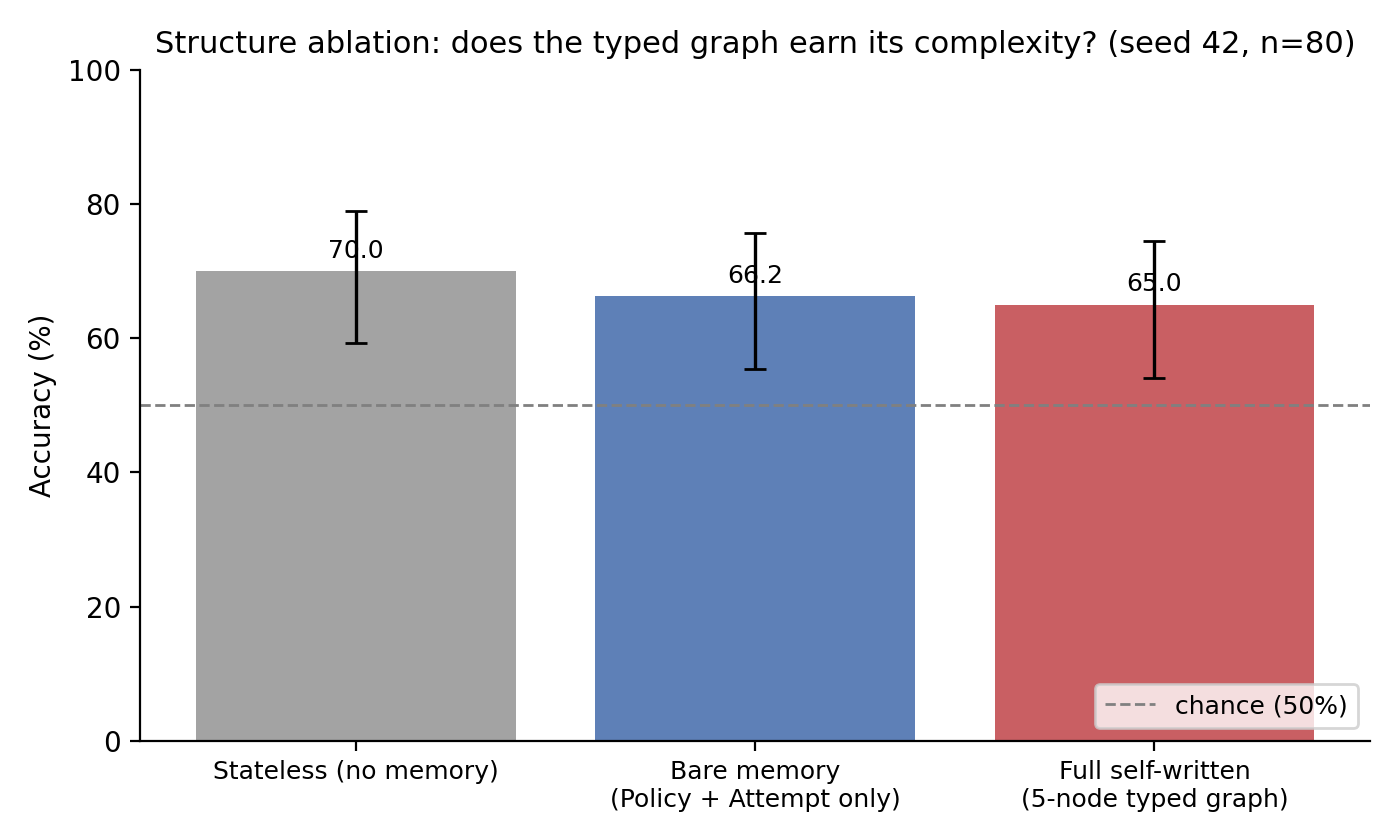
\includegraphics[width=0.8\textwidth]{figures/structure_ablation.png}
\caption{Structure ablation: accuracy of the stateless baseline, a bare Policy-plus-Attempt memory, and the full five-node typed graph, with Wilson 95\% confidence intervals. The three intervals overlap.}
\label{fig:ablation}
\end{figure}

Figure~\ref{fig:ablation} shows the three overlapping intervals. The additional extraction of Issue, Fix, and Semantic nodes does not produce a measurable verdict-accuracy gain on this benchmark.

\subsection{Cross-Seed Stability}

\begin{table}[h]
\centering
\caption{Cross-seed comparison (leakage-free, audited).}
\label{tab:seed}
\begin{tabular}{lccc}
\toprule
Mode & Seed 42 & Seed 123 & Seed 7 \\
\midrule
Stateless & 70.0\% & 70.0\% & 67.5\% \\
MAJ (self-written) & 65.0\% & 67.5\% & 66.2\% \\
MAJ (oracle) & 60.0\% & 66.2\% & 66.2\% \\
\bottomrule
\end{tabular}
\end{table}

To confirm that the conclusion is not an artifact of a single split, the stateless and MAJ modes were re-run on two further random seeds, each with its own question-level split and a passing audit (Table~\ref{tab:seed}).

\begin{figure}[h]
\centering
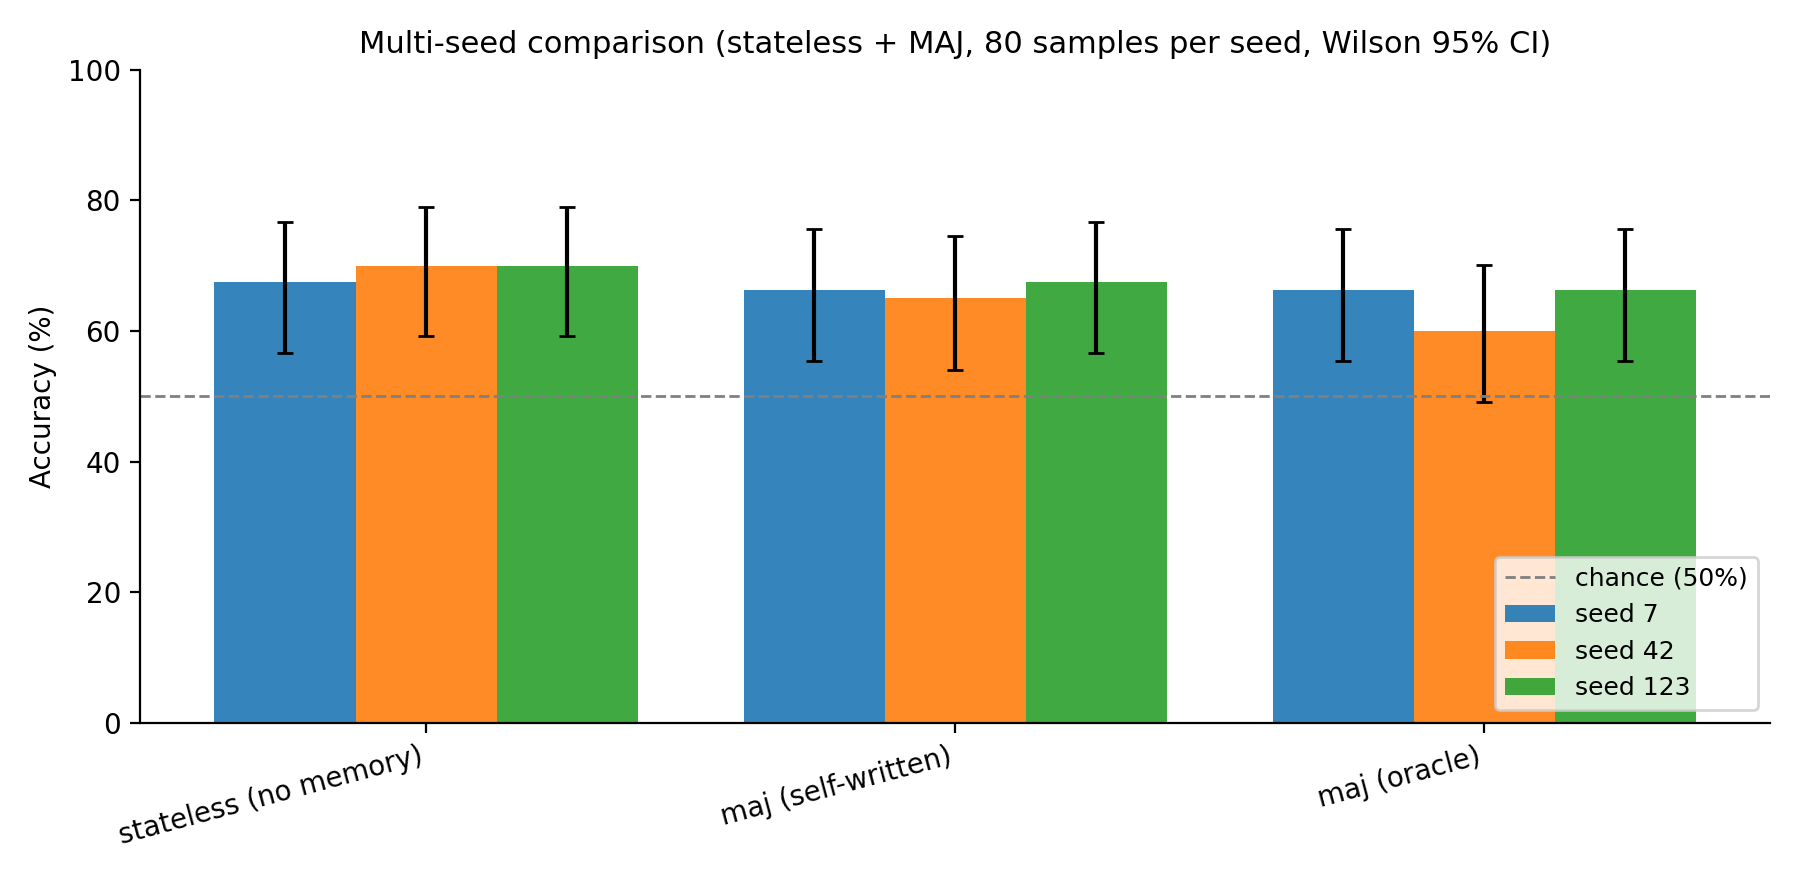
\includegraphics[width=0.95\textwidth]{figures/multiseed.png}
\caption{Cross-seed comparison of the stateless and memory-augmented modes over three random splits, with Wilson 95\% confidence intervals. The cross-seed spread of each mode is wider than the gap between modes.}
\label{fig:multiseed}
\end{figure}

As Figure~\ref{fig:multiseed} shows, across all three seeds MAJ tracks stateless within roughly two to five points and never significantly exceeds it. The per-mode range across seeds is about five points, wider than any mode-versus-mode difference on a single seed, which confirms both that the conclusion is stable and that small single-seed differences fall inside the cross-seed noise band.

\section{When Memory Appears to Corrupt: Poisoning and the Artifact}

\begin{table}[h]
\centering
\caption{Robustness to label corruption (leakage-free, audited).}
\label{tab:poison}
\begin{tabular}{lcc}
\toprule
Poison rate & MAJ & MCTS-Judge + Memory \\
\midrule
0\% (oracle) & 60.0\% & 65.4\% \\
10\% & 62.5\% & 67.5\% \\
20\% & 63.7\% & 69.7\% \\
50\% & 62.5\% & 65.4\% \\
\bottomrule
\end{tabular}
\end{table}

Under the audited protocol, neither mode degrades meaningfully as the poisoning rate rises (Table~\ref{tab:poison}). The MAJ accuracy stays within a 60--64\% band and the MCTS-Judge~+~Memory accuracy within a 65--70\% band, across all poison rates. For MCTS-Judge~+~Memory, 50\% poisoning versus oracle is a paired difference of exactly $0.0$ points (McNemar $p=1.00$).

\begin{figure}[h]
\centering
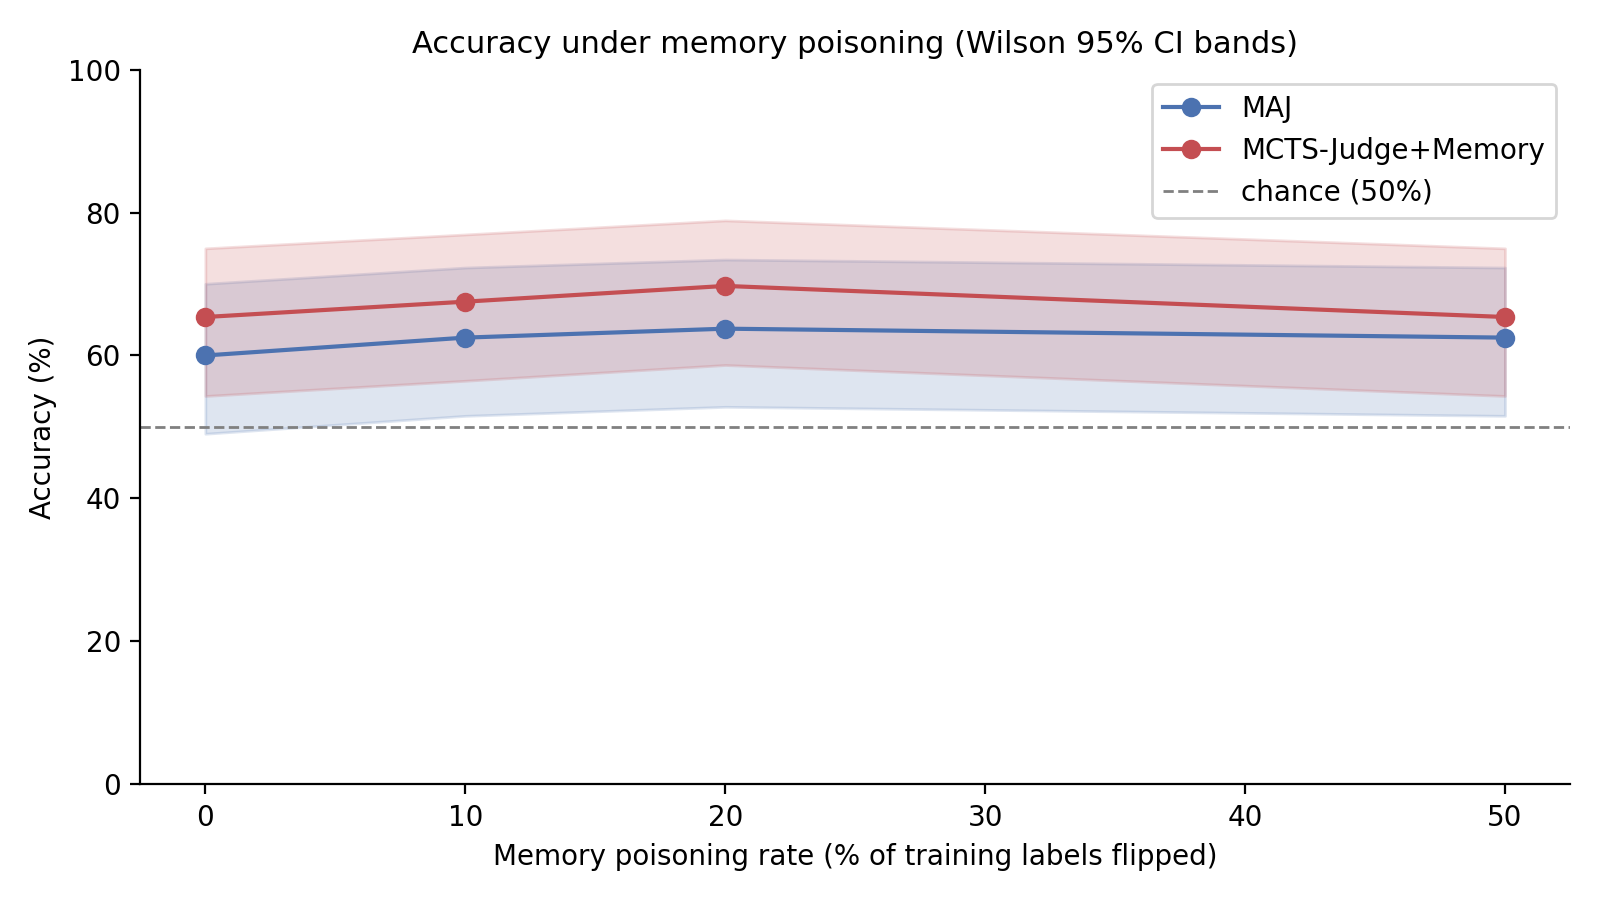
\includegraphics[width=0.95\textwidth]{figures/poisoning_curve.png}
\caption{Accuracy as a function of the memory poisoning rate, under the corrected, audited harness, with Wilson 95\% confidence interval bands. Neither mode shows a significant downward trend as the corruption rate rises.}
\label{fig:poison}
\end{figure}

Figure~\ref{fig:poison} shows the flat poisoning curves. This corrects an earlier, un-audited version of the same experiment, which reported that MCTS-Judge~+~Memory collapsed to 21.2\% accuracy at 50\% poisoning, a 48.8-point drop. That earlier run predated the transient-error correction described in Chapter~4. On inspection of the per-sample logs, the collapse was an artifact: a mid-run network outage caused a block of samples to error, and the original code recorded each errored sample as a wrong answer. Once errored samples are retried and, on persistent failure, excluded rather than counted as wrong, the 50\% poisoning condition scores 65.4\%, identical to oracle. The dramatic ``poisoning collapse'' was a property of the measurement harness, not of the system.

\section{Reliability Harness}

Beyond raw accuracy, a reliability harness probes three further properties of the judge. \emph{Stochastic stability} measures how often a mode returns the same verdict when the same item is judged twice. \emph{Label-flip discrimination} measures how often a judge correctly changes its verdict when a response is altered from passing to failing. The \emph{defense filter} tests whether a similarity-threshold filter on retrieved memory mitigates heavy poisoning. Figure~\ref{fig:harness} summarizes the results.

\begin{figure}[h]
\centering
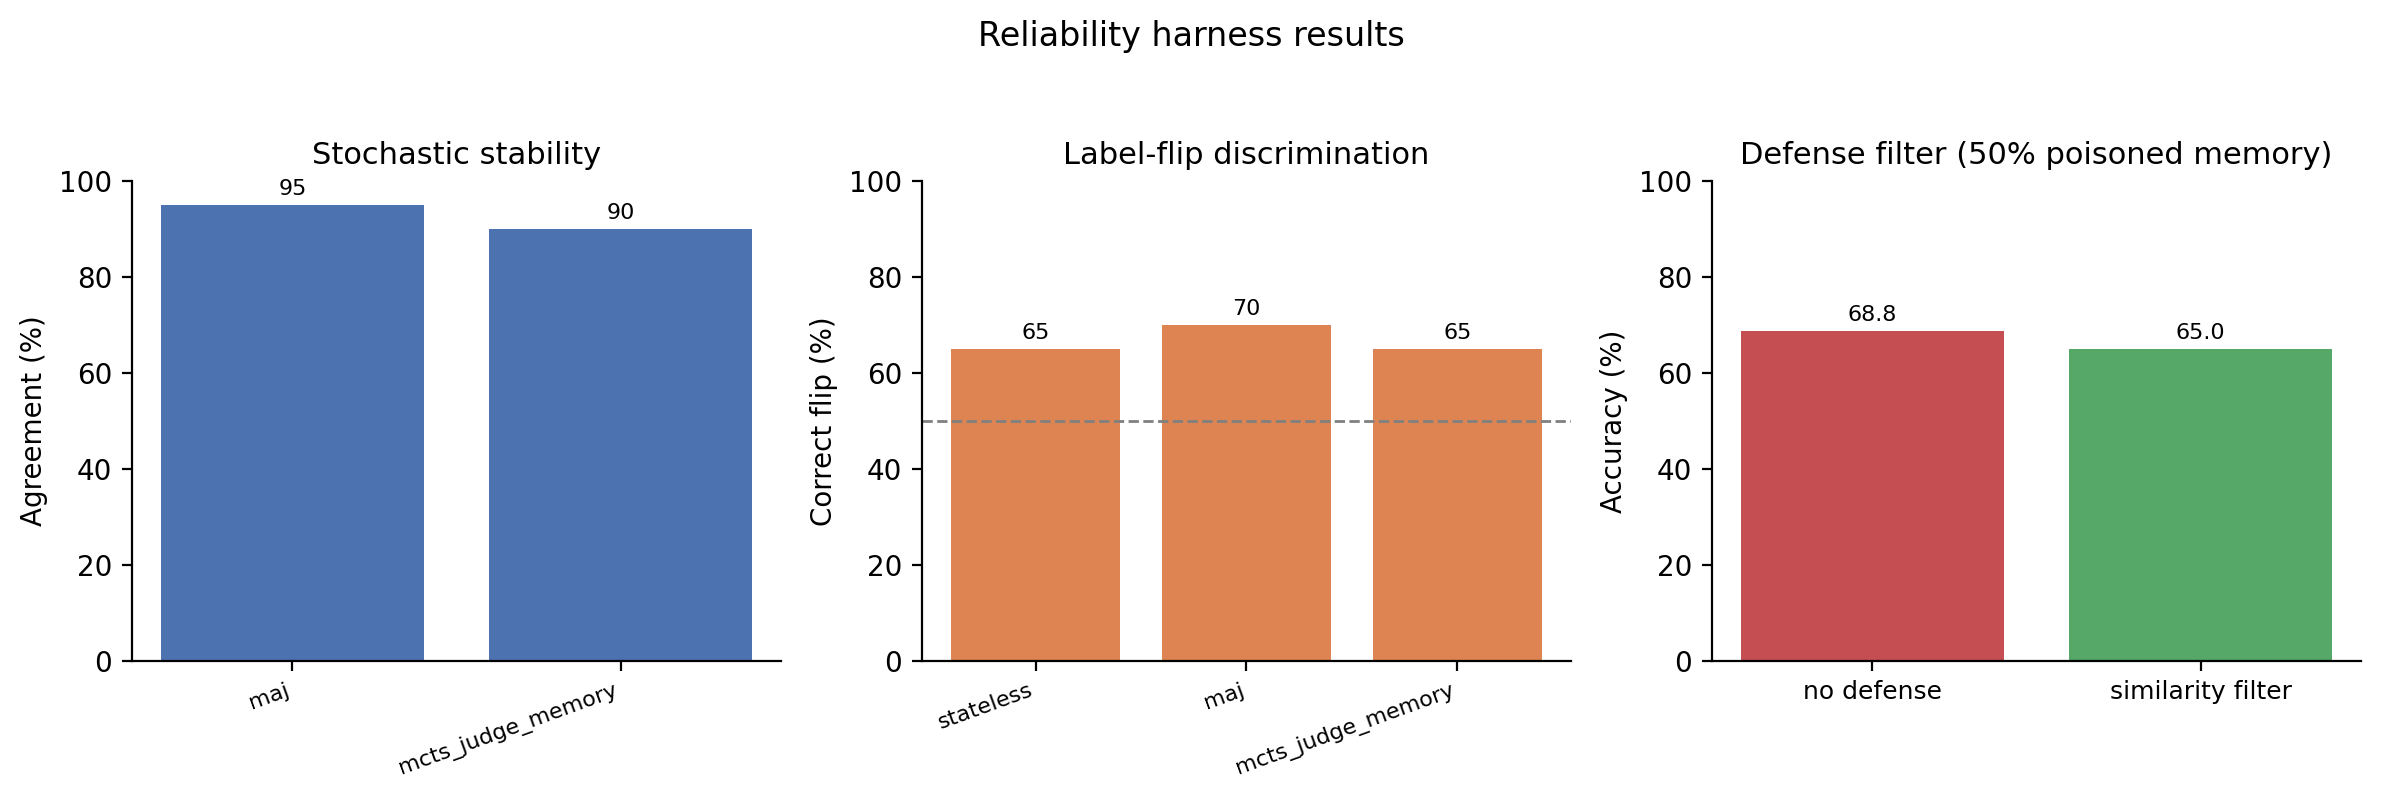
\includegraphics[width=0.95\textwidth]{figures/harness_results.png}
\caption{Reliability harness results: stochastic stability, label-flip discrimination, and the defense filter under 50\% poisoned memory.}
\label{fig:harness}
\end{figure}

Two findings are worth recording. The modes are highly stable across repeated runs, so the accuracy results above are not an artifact of stochastic noise within a single mode. The defense filter, however, does not help: under 50\% poisoned memory the filtered configuration is no more accurate than the unfiltered one. Consistent with the rest of the chapter, this is reported as an honest negative result; a defense mechanism that does not measurably mitigate the failure mode it targets should be reported as such rather than presented as a working safeguard.

\section{Discussion: Why Memory Neither Helped nor Harmed}

The experimental program gives a clear, if unglamorous, answer to the research question, and this section explains the answer mechanistically, as required for a defensible scientific verdict.

\paragraph{Why the apparent benefit disappeared.} Under a conventional protocol, memory appeared to lift the judge by six to ten points; under the leakage-free, audited protocol, no lift is detectable. The difference between the two is the evaluation protocol, not the memory system. The most parsimonious explanation is that a large part of the conventional-protocol gain was an artifact of evaluation leakage: with paired pass/fail questions and memory updated during evaluation, the judge could effectively retrieve information about the very item it was scoring. Once the question-level split and the frozen-memory audit remove both leakage channels, that information is no longer available, and the apparent gain vanishes.

\paragraph{Why memory carries no usable signal here.} Three independent results point to the same mechanism. First, oracle memory, with perfectly correct labels, does not beat self-written memory (Table~\ref{tab:oracle}); if the judge were exploiting label correctness, perfect labels would help. Second, the bare Policy-plus-Attempt memory is indistinguishable from the full five-node schema (Figure~\ref{fig:ablation}); if structured issues and fixes carried signal, removing them would hurt. Third, the cross-seed range exceeds every mode-versus-mode gap (Figure~\ref{fig:multiseed}); the differences that do appear are sampling noise. Together these indicate that GPT-4o, on graded question answering, is already operating near the ceiling its own reasoning permits: the task does not require knowledge that the model lacks, so a retrieved prior evaluation adds nothing the model could not already produce. Memory helps a judge only when it supplies information the judge does not already have; on this benchmark, it does not.

\paragraph{Why the apparent collapse disappeared.} The earlier un-audited harness reported a catastrophic accuracy collapse under heavy poisoning. The corrected, retry-instrumented harness shows no significant degradation. The collapse was caused by transient API errors being recorded as wrong answers, not by corrupted memory. This is an engineering cause with a practical fix (retry plus correct error attribution), and once fixed, the effect does not exist.

\paragraph{When memory would be expected to help.} The null result is specific to this benchmark and judge, and the mechanism above predicts when the result would change. Memory should help when the judge cannot already solve the task from its own parametric knowledge: a weaker judge model, a harder or more specialised benchmark, or tasks whose correct verdict depends on domain knowledge or on conventions established only in the memory itself. It should also help when the same or near-identical items recur, so that a retrieved past verdict is directly reusable. These are testable predictions and are the natural next experiments; they could not be settled within the scope of this thesis, but the mechanistic account makes them concrete rather than speculative.

\section{Cost of the MCTS Modes}

The MCTS modes are roughly nine to thirteen times slower than the single-pass modes: a stateless evaluation averages 3.6 seconds per sample and MAJ 4.5 seconds, whereas MCTS-Judge averages 31.8 seconds and MCTS-Judge~+~Memory 33.3 seconds. Figure~\ref{fig:latency} plots accuracy against latency on a logarithmic scale, making the cost-reliability trade-off explicit: the MCTS modes sit an order of magnitude to the right of the single-pass modes without sitting any higher. Because the audited experiments find no significant accuracy advantage for the MCTS modes, this additional cost is not currently justified by an accuracy return, and the MCTS extension is reported as exploratory.

\begin{figure}[h]
\centering
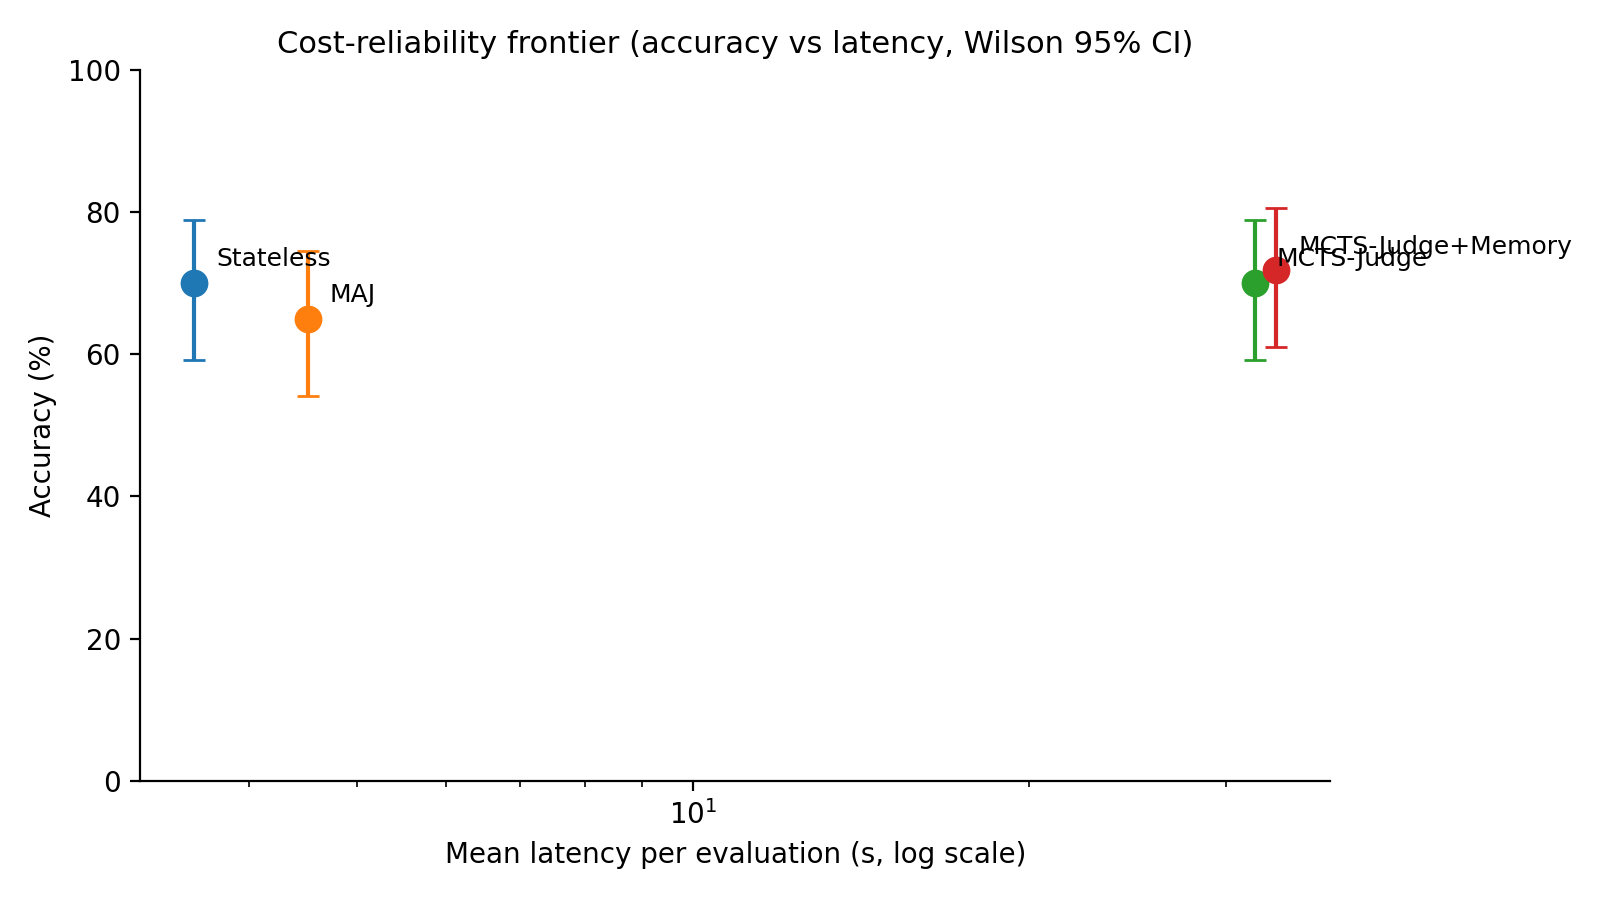
\includegraphics[width=0.95\textwidth]{figures/latency_accuracy.png}
\caption{Cost-reliability frontier: accuracy against mean latency per evaluation (logarithmic scale), with Wilson 95\% confidence intervals. The MCTS modes cost roughly an order of magnitude more latency without a corresponding accuracy gain.}
\label{fig:latency}
\end{figure}

\section{Threats to Validity}

\begin{itemize}
    \item \textbf{Sample size.} The held-out set has 80 samples; the conclusion is a null result, which at this sample size means no effect was detected, not that none exists. A larger benchmark could reveal a small genuine effect.
    \item \textbf{Single judge model.} The audited experiments use GPT-4o only; other models may behave differently, as the discussion above makes explicit.
    \item \textbf{Single benchmark.} EvalsBench is graded question answering; the conclusions are stated for that domain.
    \item \textbf{Single poisoning pattern.} Only uniform random label flipping was tested; structured adversarial poisoning may differ.
    \item \textbf{Conventional-protocol evidence.} The conventional-protocol per-sample logs were not retained, so those numbers are treated as a motivating observation rather than a verified claim.
\end{itemize}

% =====================================================================
%  CHAPTER 6 -- CONCLUSION
% =====================================================================
\chapter{Conclusion}

\section{Summary of the Work}

This thesis investigated whether a persistent, structured memory improves an LLM-as-a-Judge, and how such a system can be evaluated without leakage. A memory-augmented judging system, MCTS-MAJ, was designed and implemented, comprising a typed Neo4j memory graph, a retrieval-conditioned single-pass judge, and two exploratory Monte Carlo Tree Search components. A leakage-free evaluation protocol was designed, splitting the benchmark by question and freezing memory during testing, and a two-layer frozen-memory audit was implemented to prove, for every run, that memory was not modified during evaluation.

\section{Answer to the Research Question}

The research question asked when persistent memory helps an LLM judge, when it fails or corrupts the evaluation, and how a memory-augmented judge can be evaluated in a provably leakage-free way.

\emph{When memory appears to help.} Under a conventional protocol, memory appeared to deliver large gains. Under the leakage-free, audited protocol, those gains do not survive: on the studied benchmark no memory-augmented or tree-search configuration significantly outperforms a single-pass stateless judge, and this holds across three random seeds. The apparent benefit of memory was, to a large extent, an artifact of evaluation leakage.

\emph{When memory fails to help, and why.} Memory does not help when the judge can already solve the task from its own reasoning. Oracle memory does not beat self-written memory, the bare graph does not lose to the full schema, and the differences that appear are within cross-seed noise. Together these show that, for GPT-4o on graded question answering, the memory channel carries no verdict signal the model did not already have.

\emph{When memory appears to corrupt, and why that is misleading.} An un-audited harness reported a catastrophic accuracy collapse under heavy memory poisoning. Under a corrected, retry-instrumented harness, no significant degradation occurs; the collapse was an artifact of mishandled transient errors.

\emph{How to evaluate a memory-augmented judge without leakage.} The contribution that holds is methodological: the question-level partition, the frozen memory, and the two-layer frozen-memory audit together form a protocol that proves the absence of leakage rather than assuming it. During development this audit caught a genuine leakage defect, which demonstrates its practical value.

The overall conclusion is that, on this benchmark, both the apparent benefit and the apparent fragility of memory in LLM-as-a-Judge evaluation are largely artifacts of the evaluation protocol, and that a leakage-free, audited protocol is a necessary precondition for any trustworthy claim about memory-augmented judging.

\section{Contributions}

The thesis makes the following contributions: the design and implementation of MCTS-MAJ, a memory-augmented LLM-as-a-Judge system built on a typed Neo4j graph of past evaluations, with a three-stage retrieval pipeline and two exploratory Monte Carlo Tree Search components; a leakage-free evaluation protocol for memory-augmented LLM judges; a two-layer frozen-memory audit that proves the absence of memory leakage; an empirical finding, obtained under that protocol, that memory does not produce a statistically significant gain on the studied benchmark; a mechanistic explanation of that finding; and a methodological demonstration that an un-audited harness can report both gains and failures that do not exist.

\section{Future Work}

Several directions follow naturally. The benchmark should be enlarged well beyond 80 test samples, so that a small genuine effect, if one exists, could be resolved. The audited protocol should be applied to weaker and stronger judge models and to harder task domains, directly testing the prediction that memory helps when the judge cannot already solve the task. The leakage-free protocol and the frozen-memory audit could be packaged as a standalone, reusable evaluation tool. Finally, the structured memory graph, which did not improve verdict accuracy here, may still be valuable for interpretability and debugging, and that use deserves separate study.

\section{Concluding Remark}

The result of this thesis is a negative empirical finding paired with a positive methodological one. Memory did not measurably improve the judge; but the protocol built to test that question, and to catch the leakage and the artifacts that would otherwise have hidden the truth, is a reusable instrument, and the discipline it enforces is the lasting lesson of the work.

% =====================================================================
%  BIBLIOGRAPHY
% =====================================================================
\bibliographystyle{unsrt}
\bibliography{references}
\addcontentsline{toc}{chapter}{References}

% =====================================================================
%  APPENDICES
% =====================================================================
\appendix

\chapter{Frozen-Memory Audit Record Format}

Each evaluation run produces a machine-readable audit record that proves the memory graph was not modified during evaluation. The record stores the before-and-after snapshots and their difference. A snapshot contains the per-type node counts, the per-type relationship counts, the total node and edge counts, and a SHA-256 fingerprint over the sorted node identifiers and edge triples. A run is reported as leakage-free only if the difference is empty and the two fingerprints are identical. For a passing run the difference flag is true, both delta maps are empty, and the before and after fingerprints match exactly. Every leakage-free experiment reported in Chapter~5 has a passing record of this form, and the records are released with the source code so that the absence of leakage can be checked independently.

\chapter{Evaluation Modes and Memory Conditions}

\begin{table}[h]
\centering
\caption{Evaluation modes.}
\label{tab:appmodes}
\begin{tabular}{lll}
\toprule
Mode & Memory & Reasoning layer \\
\midrule
Stateless & none & single-pass judge \\
MAJ & three-stage retrieval & single-pass judge \\
MCTS-Judge & none & MCTS over subtasks \\
MCTS-Judge + Memory & three-stage retrieval & MCTS over subtasks \\
\bottomrule
\end{tabular}
\end{table}

\begin{table}[h]
\centering
\caption{Memory-building conditions.}
\label{tab:appcond}
\begin{tabular}{ll}
\toprule
Condition & What is stored \\
\midrule
No memory & nothing; the graph is empty \\
Self-written & the judge's own verdicts, reasoning, issues, and fixes \\
Oracle & the dataset ground-truth labels, stored directly \\
Poisoned (10/20/50\%) & oracle memory with a fixed fraction of labels flipped \\
\bottomrule
\end{tabular}
\end{table}

\chapter{Full Per-Mode Results}

Table~\ref{tab:appfull} collects every audited result in one place, with Wilson 95\% confidence intervals and the number of completed samples. Where the completed count is below 80, the remaining samples errored after retries and were excluded from the accuracy computation, as described in Chapter~4.

\begin{table}[h]
\centering
\caption{Complete audited results (GPT-4o, seed 42).}
\label{tab:appfull}
\begin{tabular}{lcc}
\toprule
Configuration & Accuracy [95\% CI] & Completed $n$ \\
\midrule
Stateless & 70.0\% [59.2, 78.9] & 80 \\
MAJ, self-written & 65.0\% [54.1, 74.5] & 80 \\
MAJ, oracle & 60.0\% [49.0, 70.0] & 80 \\
MAJ, poison 10\% & 62.5\% [51.5, 72.3] & 80 \\
MAJ, poison 20\% & 63.7\% [52.8, 73.4] & 80 \\
MAJ, poison 50\% & 62.5\% [51.5, 72.3] & 80 \\
MCTS-Judge, no memory & 70.0\% [59.2, 78.9] & 80 \\
MCTS-Judge + Memory, self-written & 71.8\% [61.0, 80.6] & 78 \\
MCTS-Judge + Memory, oracle & 65.4\% [54.3, 75.0] & 78 \\
MCTS-Judge + Memory, poison 10\% & 67.5\% [56.5, 76.9] & 77 \\
MCTS-Judge + Memory, poison 20\% & 69.7\% [58.7, 78.9] & 76 \\
MCTS-Judge + Memory, poison 50\% & 65.4\% [54.3, 75.0] & 78 \\
\bottomrule
\end{tabular}
\end{table}

\chapter{Reproduction}

All numbers, tables, and figures in this thesis are reproducible from the released source code. A single reproduction script builds memory for each condition, runs the leakage-free evaluation with the frozen-memory audit enabled, recomputes the Wilson intervals, paired bootstrap intervals, and exact McNemar tests from the per-sample files, regenerates every figure, verifies that every expected artifact and audit record is present, confirms that every audit passed, and exits with an error if any artifact is missing or any audit failed.

\end{document}
